\documentclass[letterpaper,fleqn]{article}
\usepackage[spanish,es-noshorthands]{babel}
\usepackage[utf8]{inputenc} 
\usepackage[left=1cm, right=1cm, top=1.5cm, bottom=1.7cm]{geometry}
\usepackage{mathexam}
\usepackage{amsmath}
\usepackage{graphicx}

\ExamClass{
\includegraphics[height=16pt]{Images/logo-sed.png} Álgebra $8^{\circ}$}
\ExamName{Sustentación Recomendaciones III}
\ExamHead{
\includegraphics[height=16pt]{Images/logo-colegio.png} IEDAB}
\newcommand{\LineaNombre}{%
\par
\vspace{\baselineskip}
Nombre:\hrulefill \; Curso: \underline{\hspace*{48pt}} \; Fecha: \underline{\hspace*{2.5cm}} \relax
\par}
\let\ds\displaystyle

\begin{document}
\ExamInstrBox{
Respuesta sin justificar mediante procedimiento no será tenida en cuenta en la calificación. Escriba sus respuestas en el espacio indicado.}
\LineaNombre
\begin{enumerate}
 \item Encuentre el polinomio que representa el área superficial del solido rectangular de la figura (Recuerde que \'{e}ste es un paralelep\'{i}pedo de 6 caras rectangulares)
\begin{center}
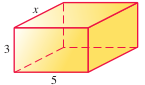
\includegraphics[scale=1]{Images/solido01.png} 
\end{center}
\noanswer
Ahora use el polinomio obtenido para determinar la superficie de los sólidos cuyas dimensiones se especifican:
\begin{enumerate}
\item 3 por 5 por 4\noanswer
\item 3 por 5 por 13\noanswer
\end{enumerate}
\item Encuentre los siguientes productos
\begin{enumerate}
\item $(-2x^{2})(6x^{3})$\noanswer
\item $(3x)(-2x^{2})(-5x^{3})$\noanswer
\item $(\frac{2}{3}xy)(-3x^{2}y)(5x^{4}y^{5})$\noanswer
\item $(12y)(-5x)(-\frac{5}{6}x^{4}y)$\noanswer
\end{enumerate}
\item Eleve cada potencia indicada
\begin{enumerate}
\item $(-2xy^{2})^{3}$\noanswer
\item $(-5a^{2}b^{2}c)^{3}$\noanswer
\end{enumerate}
\item Encuentre cada cociente
\begin{enumerate}
\item $\dfrac{25x^{5}y^{6}}{-5x^{2}y^{4}}$\noanswer
\item $\dfrac{-72x^{2}y^{4}}{-8x^{2}y^{4}}$\noanswer
\end{enumerate}
\item Multiplique los polinomios. Recuerde que puede usar la propiedad distributiva o los productos notables vistos.
\begin{enumerate}
\item $9a^{3}(2a-3b+7ab)$\noanswer
\item $(t-s)(x+y)$\noanswer
\item $(x+2)(x+10)$\noanswer
\item $(t+13)^{2}$\noanswer
\item $(5y-2)(5y+2)$\noanswer
\end{enumerate}
 \end{enumerate}

\end{document}
